\chapter{Spatial Web Crawler}
Our first step to building the platform Geo-Service portal is to gather the required spatial data. This can be done by finding the available data sources for geo-registries from the web via crawling or adding the sources manually. Spatial data is not indexed and available as compared to normal image or text data. The crawler module crawls the open web to find OGC compliant geoservers and stores their metadata information. It uses ontology or hierarchical mapping or spatial data to classify the crawled features. This features are permanently mapped into ontology to help in query processing.

% ---------------------------------------------------------------
\section{Objectives}
\begin{enumerate}
\item Build a spatial web crawler which crawlers through available geo-servers which offers WFS
based OGC compliant services.
\item Build a domain specific vocabulary(ontology) for this features which can be helpful to
compare found features with wanted features.
\item Perform semantic matching of found features from crawled web-pages with given
ontology for filtering the correct features and storing them in the permanent repository.
\item Perform an evaluation of the given spatial web crawler using metrics and test URL seed
sets.
\end{enumerate}

% ---------------------------------------------------------------

\section{Architecture of the Spatial Web Crawler}
Our crawler contains three modules for crawling spatial features through the world wide web.
Some of the definition needed for understanding the working of spatial web crawler are:\\

\begin{figure}[h]
  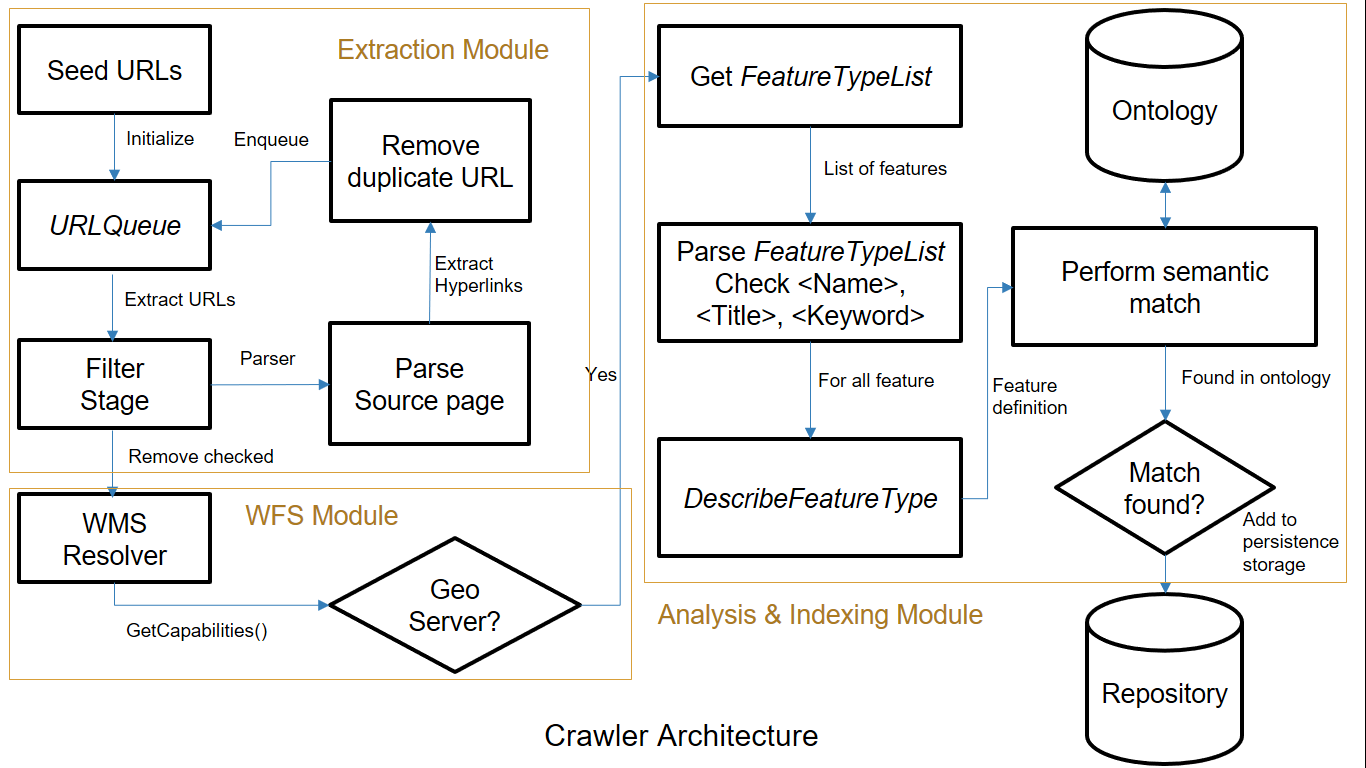
\includegraphics[width=\textwidth]{2}
  \caption{Spatial web crawler architecture}
\end{figure}


\begin{itemize}

\item  \textbf{Seed set}\\ A set of test URL(s) to initialize the queue for crawling the web. The crawler
starts with the URLs given in the seed URL set. Seed set URL(s) are processed and parsed to obtain other URL(s), which are added to the queue for later crawling.

\item \textbf{URLQueue}\\
A queue that contains set of URLs to be crawled. The crawler module takes URLs one after the another from this queue. It contains list of all the valid URL(s) to be crawled. It contains seed set initially. URL(s) are taken one by one by the crawler module for processing and deleted from the URLQueue. Similarly, newly found URL(s) are added to the queue.

\item \textbf{Frontiers}\\ 
A set of URLs from the URLQueue that are currently being crawled. This are
called frontiers because they reside between the known web and the unknown web. This are active URL(s) currently participating in the process of crawling. Frontiers are checked by the WMS resolver module for their geo-capabilities and parsed by extraction module to get new set of URL(s) to add in URLQueue.

\item \textbf{WMS resolver}\\
WMS resolver is a module that checks that if a server is WMS server
or not given the URL from the URLQueue. It uses special request URL to check whether the server replies to the URL in an OGC compliant manner. 

\item \textbf{Parser}\\
Parser is a module that downloads the webpage from the given URL and parse
the HTML webpage looking for pre-specified tags and names. After parsing it gets a
set of tags and its contents. In our implementation we parse the webpage and look for
the anchor tags within it and store all the hyperlinks from the crawled webpage. This links are then stored in the URLQueue for further processing.

\item \textbf{Ontology}\\ 
Ontology is a semantic dictionary containing all the features its type and relationship
hierarchy between features. This is used while mapping features to it's corresponding super-type and while query processing that contains more than one feature type. For example, getting overlap or intersection between two feature types.

\end{itemize}
Spatial Web Crawler is designed to contain three modules. This modules are namely Extraction module, WFS module and Analysis \& Extraction module. They are designed in a manner that they can work independently, which will come useful while implementing this as a extension in cloud based environments. :

\begin{itemize}

\item \textbf{Extraction module}\\
Our algorithm starts with a set of seed URLs contained in the seed set. We initialize the
URLQueue with these seed URLs. Initialization is done manually. It is required to choose these seed set URL(s) carefully, to get better results in crawling. Ideally, seed URLs should be good authorities, they should point to large number of good geoserver(s). Depending on the seed set, the crawler module may find more and less no of good spatial repositories in less or more amount of time. The crawler takes URL from the URLQueue and feeds it into filter stage. The filter stage takes the URL and checks
whether the given URL is already crawled or not. After filtering such URLs, they are sent to
the parser. The parser downloads the web-page from the given URL and parses it for finding
hyperlinks contained in it. These hyperlinks again go to filter stage for finding whether the
given URLs are already crawled or not. After filtering these URLs are added to the end of
URLQueue. The filtered URLs are also passed to the WFS module.\\

\item \textbf{WFS module}\\
Once the URL is fed into WFS module for the examination, WFS module sends a GetCapabilities() request to that server.
We do this by appending the request to the URL.
\begin{center}
$?
  service=wfs\&
  version=1.1.0\&
  request=GetCapabilities$
\end{center}
The server replies for this request. If the reply contains WFS\_Capabilities tag, then it offers
WFS service. We parse the received response for finding the WFS\_\\Capabilities tag. The server replies in XML format usually called capabilities.xml file, this files contains all metadata information about the feature services offered by the WFS server like number of layers, type of operations supported, feature description, etc. If the given
server is WFS server then the given URL is passed to analysis and indexing module.\\
\item \textbf{Analysis and Extraction module}\\
In this stage server response is parsed for the tag FeatureTypeList. FeatureTypeList
contains list of features. This features are stored under the tag FeatureType. FeatureType
tag contains set of keyword, title, name tags. Each of this tags are checked to see if it
contains any word from the ontology. For each of such tag found, DescribeFeatureType request
is appended to the URL.

\begin{center}
$“?service=WFS\&version=1.1.0\&request=DescribeFeatureType\&typename="+keyword$
\end{center}

Here the keyword is the name of the feature. Each of this retrieved feature is checked again
the ontology, if similar feature is found in the ontology then it is added to permanent storage in
the repository. Matching is done semantically via ontology. 
\end{itemize}

\section{Algorithm}
The \textit{Extraction algorithm} is used to crawl and parse webpages. It parses the available URL by downloading the webpage and extracts the anchor tags and corresponding URL(s) associated with it. It passes these URL(s) to \textit{WMS Resolver} module.
\newline
\begin{algorithm}[H]
	\caption{\em Extraction Algorithm }
	\textbf{Input:} set of URLs to start crawling \\
	\textbf{Output:} set of WMS capable URLs 
	%\begin{minipage}{\linewidth}
	\begin{algorithmic}[1]	 
	
	\algnewcommand{\Initialize}[1]{%
        \State \textbf{Initialize:}
        \Statex \hspace*{\algorithmicindent}\parbox[t]{.8\linewidth}{\raggedright #1}
        \newline
    } 
    
    \Initialize{
        \FOR{ URL in Input}
            \State $URLQueue.insert(URL)$
        \ENDFOR
    }
        
    \FOR{URL in URLQueue} 
        \IF{! filter(URL)}
            \STATE $preUrlSet \gets parser(URL)$
            \STATE $urlSet \gets filterDuplicate(preUrlSet)$
            \State $URLQueue.insert(urlSet)$
        \ENDIF
        \State $WMSresolver(URL)$
    \ENDFOR 
	\end{algorithmic}
\end{algorithm}
\par \textit{WMS Resolver} module checks if the URL provided by the \textit{Extraction algorithm} corresponds to a spatial repository or not. It does this via making standard OGC web service calls to the given URL. If The URL is found to be a spatial repository it is then forwarded to the Analysis and Indexing module. No actions are taken otherwise.
\newline
\begin{algorithm}[H]
    \caption{\em WMS Resolver Algorithm }
    \textbf{Input:} URL to check for OGC compliant services \\
	\textbf{Output:} WMS capabilities
	
	\begin{algorithmic}[1]
    \State $Response \gets GetCapabilities(URL)$
    \IF{$Response$ contains $WMS\_Capabilities$}
        \State $Analyze(URL)$
    \ENDIF
    \end{algorithmic}
    % \addtocounter{algorithm}{-1}
\end{algorithm}
\par The aim of \textit{Analysis \& Indexing} algorithm is to retrieve and store spatial features from the given URL. The algorithm first makes a request to get all \textit{FeatureTypes} from the spatial repository. For each \textit{FeatureType} it checks if the type matches semantically with the ontology. Matched features are stored into the repository.
\newline
\begin{algorithm}[H]
    \caption{\em Analysis \& Indexing Algorithm }
    \textbf{Input:} WFS capable URL \\
	\textbf{Output:} WFS records
	
	\begin{algorithmic}[1]
	    \State $FeatureTypeList \gets GetFeatureTypeList$
	    \FOR{ $feature in FeatureTypeList$}
	        \State $name \gets feature.name$
	        \State $description \gets DescribeFeatureTypeList(feature)$
	        
	        \IF{ $(name,description)$ matches in $ontology$}
	            \State Store record in repository
	        \ENDIF
	        
	    \ENDFOR
	\end{algorithmic}
\end{algorithm}

\section{Example Scenario \& Results}
Suppose we search for a example query after building the system. Let this query be \textit{river and snow}. Now if we search this on normal search engines like Google, it will show us results containing either river or snow. But as we have information about spatial context in this crawler. Repositories have stored the information about which features are in near proximity to each other.
\newline
\par
Other than this, we have a object ontology. Which is a hierarchical graph based on the spatial features. This graph contains generalized and specialized features. For example it suggests that river comes under the type stream which intern comes under the geometry type waterbody. This type of hierarchical classification helps us to understand the geospatial data and their features and relationships correctly. Our query is river and snow. The crawler searches the repository for finding both features river and snow or their similar representation by doing a semantic matching over ontology. Once found it can see which is the geo server which offers both of the geo services and feature types. Based on its finding from the repository we conclude our results and send the reply back to the user.
\newline
\begin{figure}[h]
    \centering
    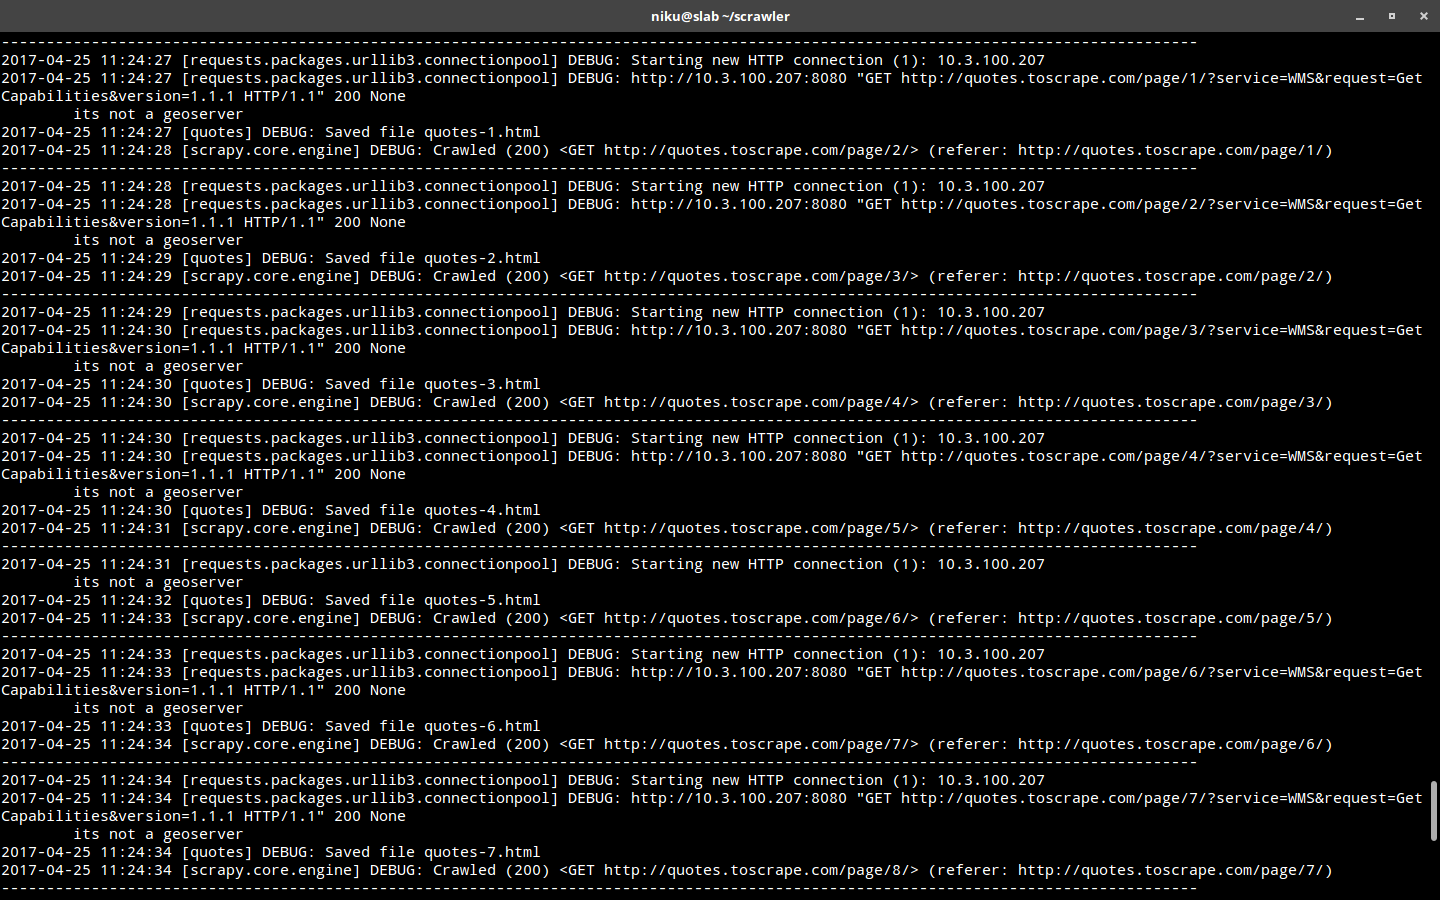
\includegraphics[width=\textwidth]{pix/p14}
    \caption{Spatial Web Crawler Implementation}
    \label{3.3}
\end{figure}
\newline
\par
Spatial web crawler is implemented with the help of Scrapy(\textit{https://scrapy.org/}) framework. It is a very powerful tool to crawl and scrap web pages. For each crawled URL, we pass it on the \textit{WMS\_Resolver} module to check if it is a spatial repository or not. Spatial GeoServer or catalog servers replies to GetCapabilities request with an XML file, part of which can be seen in the figure \ref{3.2}.
\newline
%%%%%%%%%%%%%% figure %%%%%%%%%%%%%%%%%%%%%
\begin{figure}[h]
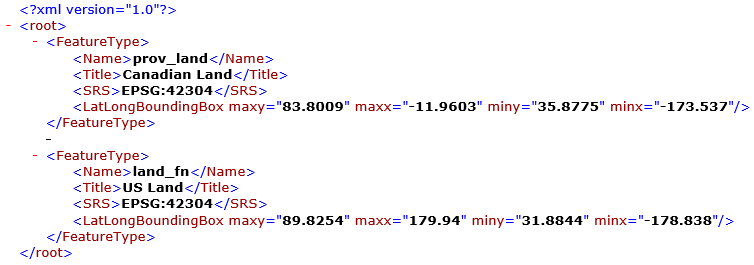
\includegraphics[width=\textwidth]{1}
\begin{center}
\caption{XML response from the geo server}
\label{3.2}
\end{center}  
\end{figure}
%%%%%%%%%%%%% figure end %%%%%%%%%%%%%%%%%%
\par
If the URL is not geo spatially capable, It is skipped as shown in the figure \ref{3.3}. For each URL the script prints if the URL is a GeoServer or not. If the URL is found to be a GeoServer, the response related to it is stored as XML and is further parsed and processed by catalog server.

\section{Advantages of Spatial Web Crawler}

\begin{itemize}
\item  Allows search in web pages that are not generally searchable from the normal search
engines. This is because of the spatial context awareness of the spatial web crawler.
\item It provides more up-to-date results from the results. Spatial crawler is more sensitive to
changes of spatial data on the web and automatically crawls through the changed
features with the help of automatic update module.
\item Provides improved accuracy in the search of spatial features and operations.
\item Provides extra features such as bounding box of spatially crawled data and other spatial
features. This bounding box can then be used for visualizing the crawled data.
\item Spatial data mining and analysis kind of tasks can be performed. So that we can infer and predict new results and patterns.
\end{itemize}